\documentclass{beamer}
\usetheme{metropolis}

\title{Explainable AI}
\subtitle{Training and Testing a Neural Network}
\author{Ryan Benasutti}
\institute{Worcester Polytechnic Institute}
\date{February 28, 2019}

\graphicspath{{./figures/}}

\begin{document}

\maketitle

\begin{frame}{Research Goals}
    \begin{itemize}
        \item Experimentally demonstrate problems with bias in training data sets
        \item Show effective methods to test for trained bias
    \end{itemize}
\end{frame}

\begin{frame}{Modeling the Problem}
    Dilemma - 2+ Options

    Option - 0..10 People

    Person - Attributes: Age, Race, Jaywalking, etc.
\end{frame}

\begin{frame}{Experimental Results}
    \begin{figure}
        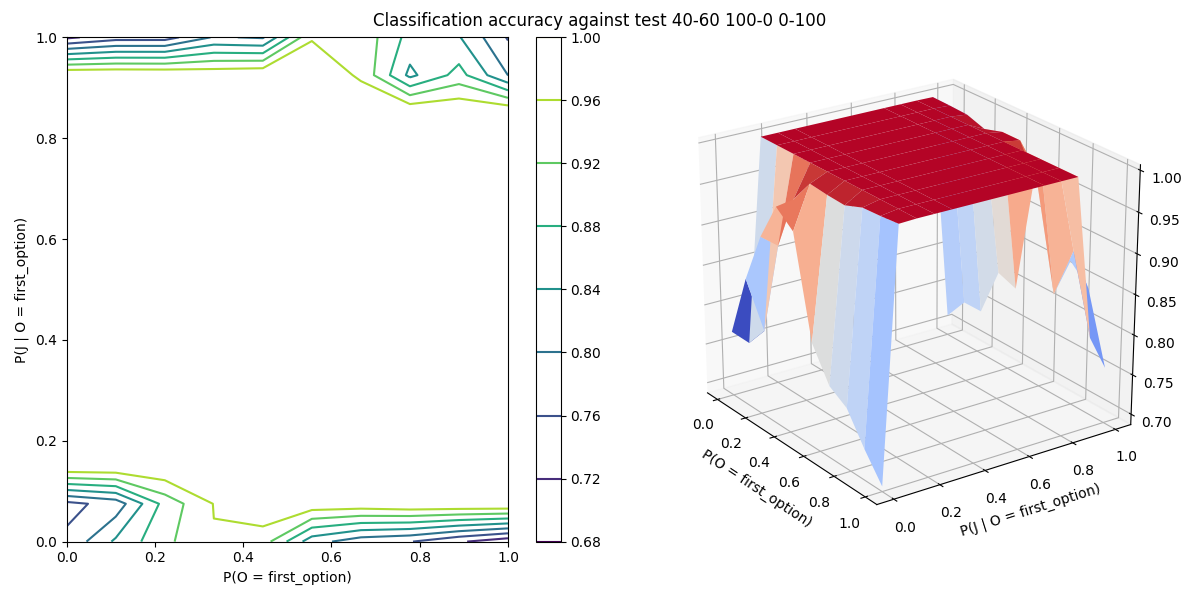
\includegraphics[scale=0.25]{test_40-60_100-0_0-100_accuracy.png}
        \caption{Classification Accuracy}
    \end{figure}
\end{frame}

\begin{frame}{Experimental Results}
    \begin{figure}
        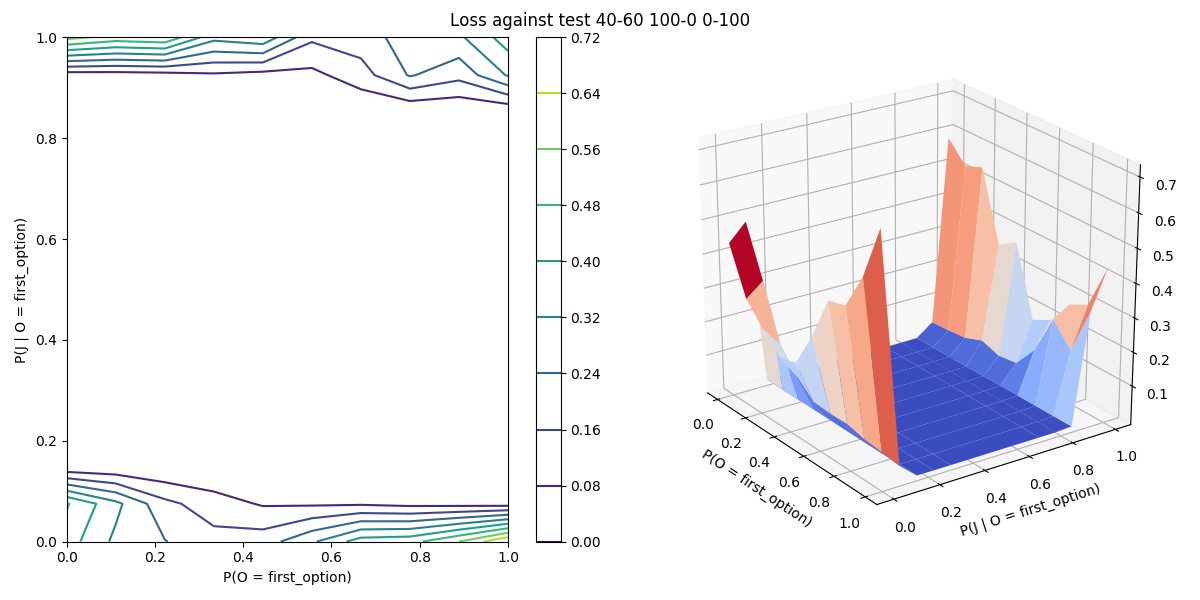
\includegraphics[scale=0.25]{test_40-60_100-0_0-100_loss.png}
        \caption{Loss}
    \end{figure}
\end{frame}

\begin{frame}{Experimental Results}
    \begin{figure}
        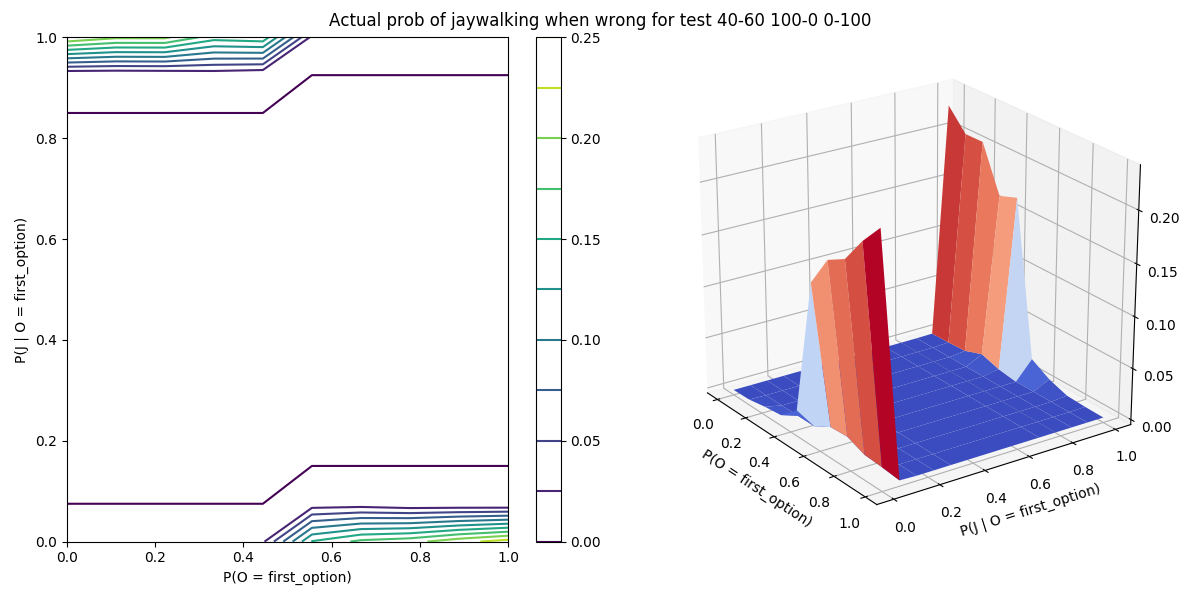
\includegraphics[scale=0.25]{test_40-60_100-0_0-100_jay_prob.png}
        \caption{Actual Jaywalking Probability}
    \end{figure}
\end{frame}

\end{document}
